

Trong quá trình xây dựng cây AST, các thành phần mã nguồn trong Rust sẽ được phân tích thành dạng cây tương ứng.
Dưới đây là một số hình ảnh ví dụ về cây AST ứng với các thành phần mã nguồn này.

\begin{figure}[H]
  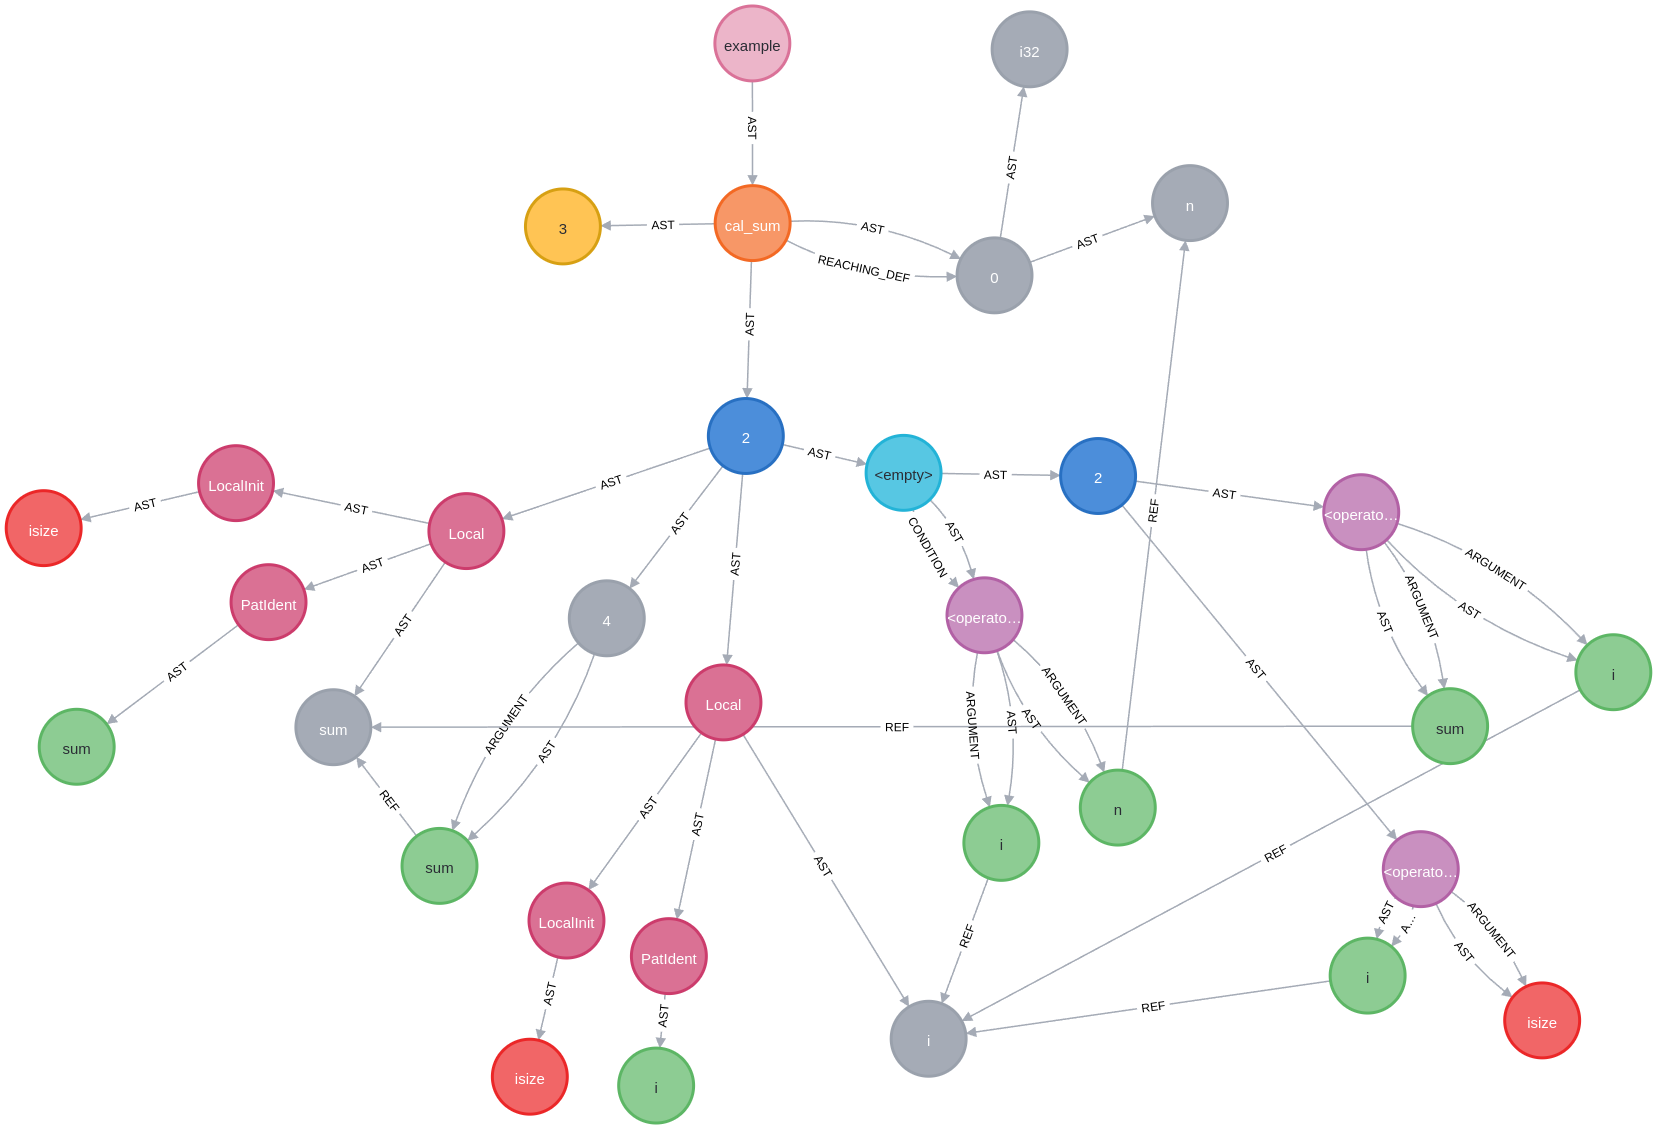
\includegraphics[width=1\columnwidth]{figures/c2/c2_cpg.png}
  \centering
  \caption{Minh họa đồ thị CPG.}
  \label{img:c3_temp1}
\end{figure}

Hình \ref{img:c3_temp1} biểu diễn một hàm được phân tích thành một nút định nghĩa hàm (FunctionDeclaration), nút này có các thuộc tính là chữ ký (signature), kiểu trả về (returnType) và tên đầy đủ (fullName).
Nút có các nút con gồm nút định danh (Identifier) biểu diễn định danh của hàm, nút kiểu hàm (FunctionType) biểu diễn kiểu dữ liệu của hàm và nút thân hàm (BlockStatement).

\begin{figure}[H]
  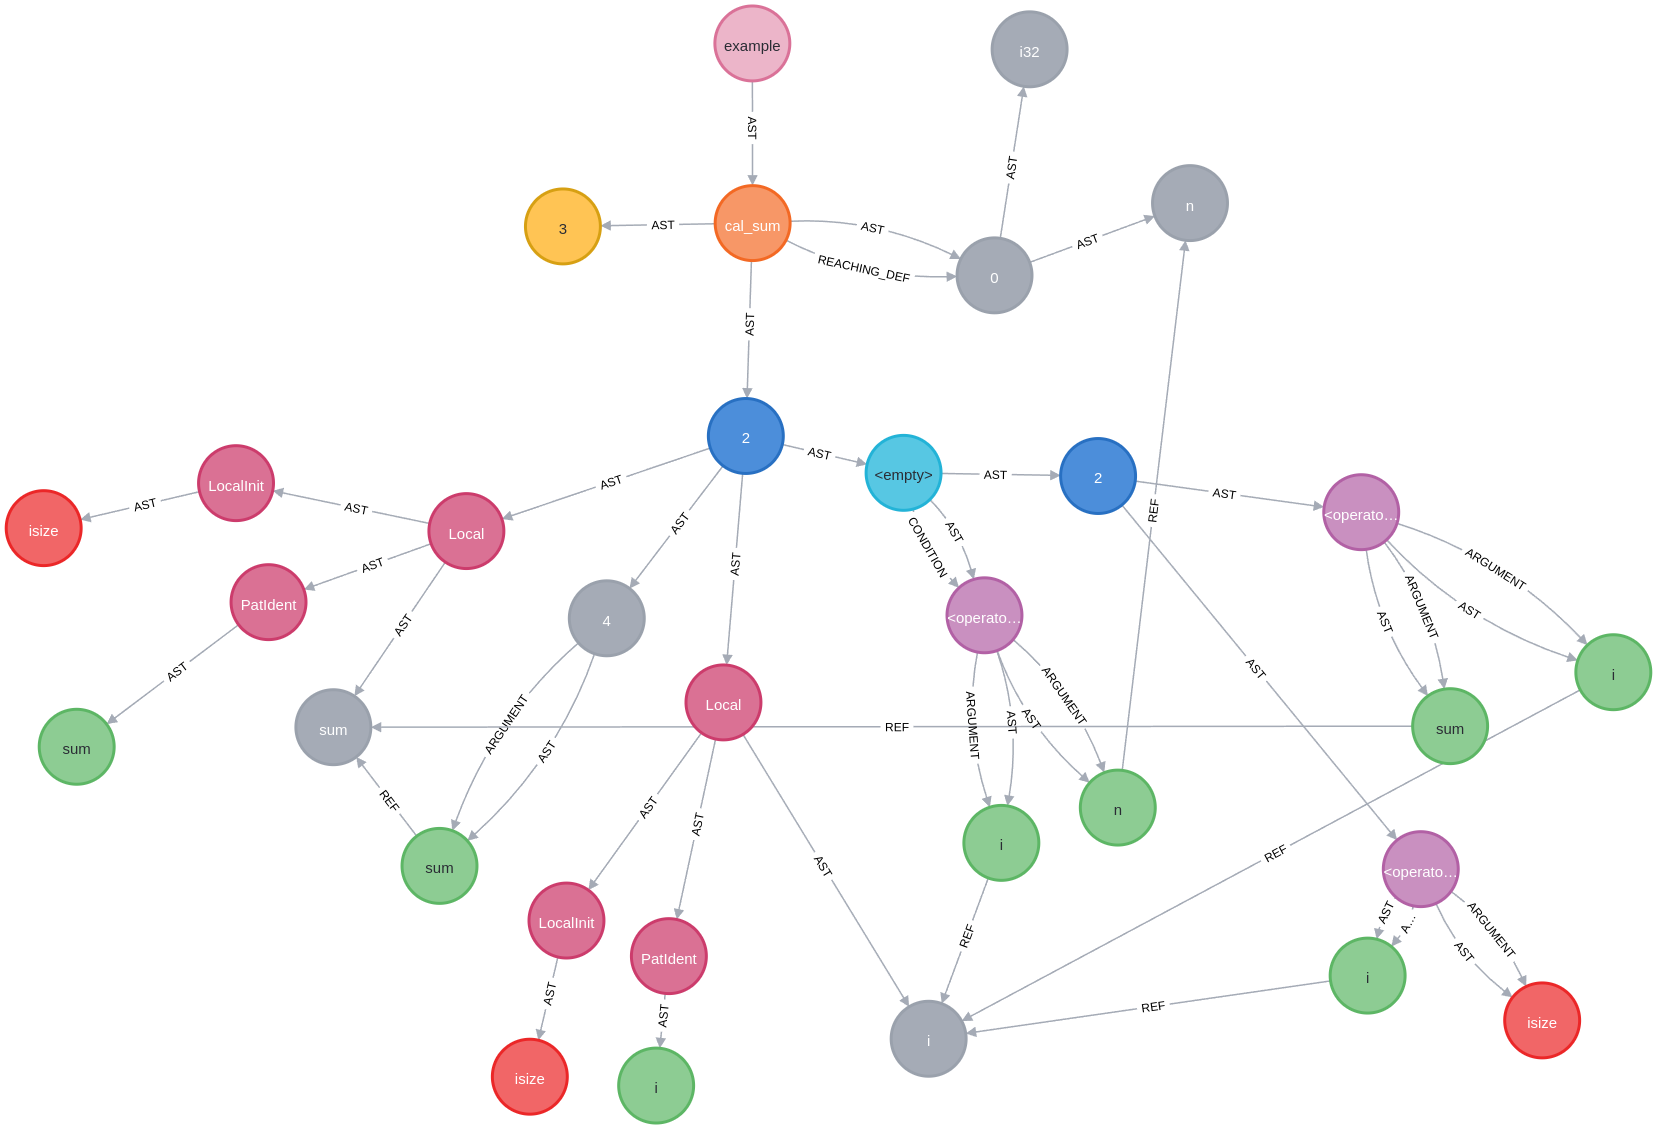
\includegraphics[width=1\columnwidth]{figures/c2/c2_cpg.png}
  \centering
  \caption{Minh họa đồ thị CPG.}
  \label{img:c3_temp2}
\end{figure}

Ví dụ về biểu diễn một kiểu cấu trúc được thể hiện trong Hình \ref{img:c3_temp2}.
Nút TypeSpecification đại diện cho định nghĩa kiểu.
Nút Identifier là nút định danh biểu diễn tên kiểu.
Nút StructType biểu diễn kiểu cấu trúc.
Nút FieldList có các nút con là Field biểu diễn các thuộc tính của kiểu này.

Các nút trong cây cú pháp mã nguồn của Rust được liệt kê trong Bảng \ref{table:c3s_nodeastrust}.

\footnotesize
\begin{longtable}{| p{.06\textwidth} | p{.31\textwidth} | p{.63\textwidth} |}
\hline
\textbf{STT} & \textbf{Tên nút} & \textbf{Mô tả} \\ \hline
1     & Abi                            & The binary interface of a function: `extern "C"`.                                                              \\ \hline
2     & \makecell{AngleBracketed \\ GenericArguments} & Angle bracketed arguments of a path segment: the `<K, V>` in HashMap<K, V>.                                    \\ \hline
3     & Arm                            & One arm of a `match` expression: `0..=10 => { return true; }`.                                                 \\ \hline
4     & AssocConst                     & An equality constraint on an associated constant: `the PANIC = false in Trait<PANIC = false>`.                 \\ \hline
5     & AssocType                      & A binding (equality constraint) on an associated type: `the Item = u8 in Iterator<Item = u8>`.                 \\ \hline
6     & Attribute                      & An attribute, like `\#[repr(transparent)]`.                                                                     \\ \hline
7     & BareFnArg                      & An argument in a function type: `the usize in fn(usize) -> bool`.                                              \\ \hline
8     & BareVariadic                   & The variadic argument of a function pointer like `fn(usize, ...)`.                                             \\ \hline
9     & Block                          & A braced block containing Rust statements.                                                                     \\ \hline
10    & BoundLifetimes                 & A set of bound lifetimes: `for<'a, 'b, 'c>`.                                                                   \\ \hline
11    & ConstParam                     & A const generic parameter: `const LENGTH: usize`.                                                              \\ \hline
12    & Constraint                     & An associated type bound: `Iterator<Item: Display>`.                                                           \\ \hline
13    & DataEnum                       & An enum input to a `proc\_macro\_derive` macro.                                                                  \\ \hline
14    & DataStruct                     & A struct input to a `proc\_macro\_derive` macro.                                                                 \\ \hline
15    & DataUnion                      & An untagged union input to a `proc\_macro\_derive` macro.                                                        \\ \hline
16    & DeriveInput                    & Data structure sent to a `proc\_macro\_derive` macro.                                                            \\ \hline
17    & Error                          & Error returned when a Syn parser cannot parse the input tokens.                                                \\ \hline
18    & ExprArray                      & A slice literal expression: `[a, b, c, d]`.                                                                    \\ \hline
19    & ExprAssign                     & An assignment expression: `a = compute()`.                                                                     \\ \hline
20    & ExprAsync                      & An async block: `async { ... }`.                                                                               \\ \hline
21    & ExprAwait                      & An await expression: `fut.await`.                                                                              \\ \hline
22    & ExprBinary                     & A binary operation: `a + b, a += b`.                                                                           \\ \hline
23    & ExprBlock                      & A blocked scope: `{ ... }`.                                                                                    \\ \hline
24    & ExprBreak                      & A `break`, with an optional label to break and an optional expression.                                         \\ \hline
25    & ExprCall                       & A function call expression: `invoke(a, b)`.                                                                    \\ \hline
26    & ExprCast                       & A cast expression: `foo as f64`.                                                                               \\ \hline
27    & ExprClosure                    & A closure expression: `[a, b] + a + b`.                                                                        \\ \hline
28    & ExprConst                      & A const block: `const { ... }`.                                                                                \\ \hline
29    & ExprContinue                   & A `continue`, with an optional label.                                                                          \\ \hline
30    & ExprField                      & Access of a named struct field `obj.k` or unnamed tuple struct field `obj.0`.                                  \\ \hline
31    & ExprForLoop                    & A for loop: `for pat in expr { ... }`.                                                                         \\ \hline
32    & ExprGroup                      & An expression contained within invisible delimiters.                                                           \\ \hline
33    & ExprIf                         & An if expression with an optional else block: if expr { ... } else { ... }.                                    \\ \hline
34    & ExprIndex                      & A square bracketed indexing expression: vector[2].                                                             \\ \hline
35    & ExprInfer                      & The inferred value of a const generic argument, denoted \_.                                                    \\ \hline
36    & ExprLet                        & A let guard: let Some(x) = opt.                                                                                \\ \hline
37    & ExprLit                        & A literal in place of an expression: 1, "foo".                                                                 \\ \hline
38    & ExprLoop                       & Conditionless loop: loop { ... }.                                                                              \\ \hline
39    & ExprMacro                      & A macro invocation expression: format!("{}", q).                                                               \\ \hline
40    & ExprMatch                      & A match expression: match n { Some(n) => {}, None => {} }.                                                     \\ \hline
41    & ExprMethodCall                 & A method call expression: x.foo::<T>(a, b).                                                                    \\ \hline
42    & ExprParen                      & A parenthesized expression: (a + b).                                                                           \\ \hline
43    & ExprPath                       & A path like std::mem::replace possibly containing generic parameters and a qualified self-type.                \\ \hline
44    & ExprRange                      & A range expression: 1..2, 1.., ..2, 1..=2, ..=2.                                                               \\ \hline
45    & ExprRawAddr                    & Address-of operation: \&raw const place or \&raw mut place.                                                      \\ \hline
46    & ExprReference                  & A referencing operation: \&a or \&mut a.                                                                         \\ \hline
47    & ExprRepeat                     & An array literal constructed from one repeated element: [0u8; N].                                              \\ \hline
48    & ExprReturn                     & A return, with an optional value to be returned.                                                               \\ \hline
49    & ExprStruct                     & A struct literal expression: Point { x: 1, y: 1 }.                                                             \\ \hline
50    & ExprTry                        & A try-expression: expr?.                                                                                       \\ \hline
51    & ExprTryBlock                   & A try block: try { ... }.                                                                                      \\ \hline
52    & ExprTuple                      & A tuple expression: (a, b, c, d).                                                                              \\ \hline
53    & ExprUnary                      & A unary operation: !x, \*x.                                                                                    \\ \hline
54    & ExprUnsafe                     & An unsafe block: unsafe { ... }.                                                                               \\ \hline
55    & ExprWhile                      & A while loop: while expr { ... }.                                                                              \\ \hline
56    & ExprYield                      & A yield expression: yield expr.                                                                                \\ \hline
57    & Field                          & A field of a struct or enum variant.                                                                           \\ \hline
58    & FieldPat                       & A single field in a struct pattern.                                                                            \\ \hline
59    & FieldValue                     & A field-value pair in a struct literal.                                                                        \\ \hline
60    & FieldsNamed                    & Named fields of a struct or struct variant such as Point { x: f64, y: f64 }.                                   \\ \hline
61    & FieldsUnnamed                  & Unnamed fields of a tuple struct or tuple variant such as Some(T).                                             \\ \hline
62    & File                           & A complete file of Rust source code.                                                                           \\ \hline
63    & ForeignItemFn                  & A foreign function in an extern block.                                                                         \\ \hline
64    & ForeignItemMacro               & A macro invocation within an extern block.                                                                     \\ \hline
65    & ForeignItemStatic              & A foreign static item in an extern block: static ext: u8.                                                      \\ \hline
66    & ForeignItemType                & A foreign type in an extern block: type void.                                                                  \\ \hline
67    & Generics                       & Lifetimes and type parameters attached to a declaration of a function, enum, trait, etc.                       \\ \hline
68    & Ident                          & A word of Rust code, which may be a keyword or legal variable name.                                            \\ \hline
69    & ImplGenerics                   & Returned by Generics::split\_for\_impl.                                                                          \\ \hline
70    & ImplItemConst                  & An associated constant within an impl block.                                                                   \\ \hline
71    & ImplItemFn                     & An associated function within an impl block.                                                                   \\ \hline
72    & ImplItemMacro                  & A macro invocation within an impl block.                                                                       \\ \hline
73    & ImplItemType                   & An associated type within an impl block.                                                                       \\ \hline
74    & Index                          & The index of an unnamed tuple struct field.                                                                    \\ \hline
75    & ItemConst                      & A constant item: `const MAX: u16 = 65535`.                                                                     \\ \hline
76    & ItemEnum                       & An enum definition: `enum Foo<A, B> { A(A), B(B) }`.                                                           \\ \hline
77    & ItemExternCrate                & An extern crate item: `extern crate serde`.                                                                    \\ \hline
78    & ItemFn                         & A free-standing function: `fn process(n: usize) -> Result<(), { ... }`.                                          \\ \hline
79    & ItemForeignMod                 & A block of foreign items: `extern "C" { ... }`.                                                                \\ \hline
80    & ItemImpl                       & \makecell{An impl block providing trait or associated items: \\ `impl<A> Trait for Data<A> { ... }`.}                        \\ \hline
81    & ItemMacro                      & A macro invocation, which includes `macro\_rules!` definitions.                                                 \\ \hline
82    & ItemMod                        & A module or module declaration: `mod m or mod m { ... }`.                                                      \\ \hline
83    & ItemStatic                     & A static item: `static BIKE: Shed = Shed(42)`.                                                                 \\ \hline
84    & ItemStruct                     & A struct definition: `struct Foo<A> { x: A }`.                                                                 \\ \hline
85    & ItemTrait                      & A trait definition: `pub trait Iterator { ... }`.                                                              \\ \hline
86    & ItemTraitAlias                 & A trait alias: `pub trait SharableIterator = Iterator + Sync`.                                                 \\ \hline
87    & ItemType                       & \makecell{A type alias: \\ `type Result<T> = std::result::Result<T, MyError>`.}                                              \\ \hline
88    & ItemUnion                      & A union definition: `union Foo<A, B> { x: A, y: B }`.                                                          \\ \hline
89    & ItemUse                        & A use declaration: `use std::collections::HashMap`.                                                            \\ \hline
90    & Label                          & A lifetime labeling a for, while, or loop.                                                                     \\ \hline
91    & Lifetime                       & A Rust lifetime: `'a`.                                                                                         \\ \hline
92    & LifetimeParam                  & A lifetime definition: `'a: 'b + 'c + 'd`.                                                                     \\ \hline
93    & LitBool                        & A boolean literal: `true or false`.                                                                            \\ \hline
94    & LitByte                        & A byte literal: `b'f'`.                                                                                        \\ \hline
95    & LitByteStr                     & A byte string literal: `b"foo"`.                                                                               \\ \hline
96    & LitCStr                        & A null-terminated C-string literal: `c"foo"`.                                                                  \\ \hline
97    & LitChar                        & A character literal: `'a'`.                                                                                    \\ \hline
98    & LitFloat                       & A floating point literal: `1f64 or 1.0e10f64`.                                                                 \\ \hline
99    & LitInt                         & An integer literal: `1 or 1u16`.                                                                               \\ \hline
100   & LitStr                         & A UTF-8 string literal: `"foo"`.                                                                               \\ \hline
101   & Local                          & A local let binding: `let x: u64 = s.parse()?`.                                                                \\ \hline
102   & LocalInit                      & The expression assigned in a local let binding, including optional diverging else block.                       \\ \hline
103   & Macro                          & A macro invocation: `println!("{}!", mac)`.                                                                    \\ \hline
104   & MetaList                       & A structured list within an attribute, like `derive(Copy, Clone)`.                                             \\ \hline
105   & MetaNameValue                  & A name-value pair within an attribute, like `feature = "nightly"`.                                             \\ \hline
106   & \makecell{Parenthesized \\ GenericArguments}  & Arguments of a function path segment: the (A, B) -> C in `Fn(A, B) -> C`.                                      \\ \hline
133   & PatConst                       & A pattern that contains a constant.                                                                            \\ \hline
134   & PatIdent                       & A pattern that matches an identifier or wildcard: `mut var @ pat`.                                             \\ \hline
135   & PatLit                         & A pattern that matches a literal value.                                                                        \\ \hline
136   & PatMacro                       & A pattern that comes from an inline macro.                                                                     \\ \hline
137   & PatOr                          & A pattern that matches any one of a list of patterns.                                                          \\ \hline
138   & PatParen                       & A pattern enclosed in parentheses.                                                                             \\ \hline
139   & PatPath                        & A pattern that matches a path to a constant.                                                                   \\ \hline
140   & PatRange                       & A pattern that matches a range of values.                                                                      \\ \hline
141   & PatReference                   & A pattern that matches a reference.                                                                            \\ \hline
142   & PatRest                        & A pattern that matches the rest pattern: `..`.                                                                 \\ \hline
143   & PatSlice                       & A pattern that matches a slice of values.                                                                      \\ \hline
144   & PatStruct                      & A pattern that matches a struct.                                                                               \\ \hline
145   & PatTuple                       & A pattern that matches a tuple.                                                                                \\ \hline
146   & PatTupleStruct                 & A pattern that matches a tuple struct.                                                                         \\ \hline
147   & PatType                        & A pattern that matches a type.                                                                                 \\ \hline
148   & PatWild                        & A wildcard pattern: `\_`.                                                                                       \\ \hline
149   & Path                           & A path like `std::mem::replace`, possibly containing generic parameters and a self-type.                       \\ \hline
150   & PathSegment                    & A segment of a path: `std`, `std::mem`, `std::mem::replace`.                                                   \\ \hline
151   & PreciseCapture                 & Specifies precise capture behavior for closures.                                                               \\ \hline
152   & PredicateLifetime              & A lifetime predicate in a where clause.                                                                        \\ \hline
153   & PredicateType                  & A type predicate in a where clause.                                                                            \\ \hline
154   & QSelf                          & The portion of a path before the `::`, if the path is qualified.                                               \\ \hline
155   & Receiver                       & The self argument of an associated method: `\&self` or `\&mut self`.                                             \\ \hline
156   & Signature                      & A function signature in a trait or impl block.                                                                 \\ \hline
157   & StmtMacro                      & \makecell{A macro invocation as a statement: \\ `println!("Hello, world!")`.}                                                \\ \hline
158   & TraitBound                     & A trait bound on a type parameter or associated type.                                                          \\ \hline
159   & TraitItemConst                 & An associated constant in a trait.                                                                             \\ \hline
160   & TraitItemFn                    & An associated function in a trait.                                                                             \\ \hline
161   & TraitItemMacro                 & A macro invocation in a trait.                                                                                 \\ \hline
162   & TraitItemType                  & An associated type in a trait.                                                                                 \\ \hline
163   & TurboFish                      & A turbo-fish, e.g., `collect::<Vec<\_>>()`.                                                                     \\ \hline
164   & TypeArray                      & An array type: `[T; n]`.                                                                                       \\ \hline
165   & TypeBareFn                     & A bare function type: `fn(usize) -> bool`.                                                                     \\ \hline
166   & TypeGenerics                   & A generic type parameter in a type definition.                                                                 \\ \hline
167   & TypeGroup                      & A group of types.                                                                                              \\ \hline
168   & TypeImplTrait                  & An `impl Trait` type in return position.                                                                       \\ \hline
169   & TypeInfer                      & An inferred type: `\_`.                                                                                         \\ \hline
170   & TypeMacro                      & A macro in the type position.                                                                                  \\ \hline
171   & TypeNever                      & The never type: !.                                                                                             \\ \hline
172   & TypeParam                      & A generic type parameter: T: Into<String>.                                                                     \\ \hline
173   & TypeParen                      & A parenthesized type equivalent to the inner type.                                                             \\ \hline
174   & TypePath                       & A path like std::slice::Iter, optionally qualified with a self-type as in <Vec<T> as SomeTrait>::Associated.   \\ \hline
175   & TypePtr                        & A raw pointer type: const T or \*mut T.                                                                        \\ \hline
176   & TypeReference                  & A reference type: \&'a Tor \&'a mut T.                                                                           \\ \hline
177   & TypeSlice                      & A dynamically sized slice type: [T].                                                                           \\ \hline
178   & TypeTraitObject                & A trait object type dyn Bound1 Bound2 + Bound3 where Bound is a trait or a lifetime.                           \\ \hline
179   & TypeTuple                      & A tuple type: (A, B, C, String).                                                                               \\ \hline
180   & UseGlob                        & A glob import in a use item: \*.                                                                               \\ \hline
181   & UseGroup                       & A braced group of imports in a use item: {A, B, C}.                                                            \\ \hline
182   & UseName                        & An identifier imported by a use item: HashMap.                                                                 \\ \hline
183   & UsePath                        & A path prefix of imports in a use item: std::..                                                                \\ \hline
184   & UseRename                      & An renamed identifier imported by a use item: HashMap as Map.                                                  \\ \hline
185   & Variadic                       & The variadic argument of a foreign function.                                                                   \\ \hline
186   & Variant                        & An enum variant.                                                                                               \\ \hline
187   & VisRestricted                  & A visibility level restricted to some path: pub (self) or pub (super) or pub (crate) or pub (in some::module). \\ \hline
188   & WhereClause                    & A where clause in a definition: where T: Deserialize<'de>, D: 'static.                                         \\ \hline
\caption{Các nút trong cú pháp mã nguồn của Rust.}
\label{table:c3s_nodeastrust}
\end{longtable}
\medskip

Mục này sẽ trình bày quá trình công cụ phân tích ánh xạ cây AST
thành đồ thị CPG.

\subsection{Các loại đỉnh và cạnh của đồ thị CPG}

Đồ thị CPG là dạng cấu trúc dữ liệu được kết hợp giữa cây AST, đồ thị CFG điều khiển và đồ thị PDG.
Đồ thị này biểu diễn các đỉnh là các nút trong cây AST và các cạnh của đồ thị biểu diễn mối quan hệ giữa chúng.
Đồ thị này giúp theo dõi các luồng điều khiển, các phụ thuộc trong mã nguồn.

Bảng \ref{table:c3_nodecpgjoern} dưới đây mô tả các đỉnh trong đồ thị CPG

\footnotesize
\begin{longtable}{| p{.06\textwidth} | p{.31\textwidth} | p{.63\textwidth} |}
\hline
\textbf{STT} & \textbf{Tên nút} & \textbf{Mô tả} \\ \hline
1   & META\_DATA         & Nút này chứa siêu dữ liệu (metadata) của đồ thị. Một đồ thị CPG phải có và chỉ có duy nhất một nút META\_DATA.                                                   \\ \hline
2   & FILE              & Nút biểu diễn một tệp mã nguồn. Với mỗi tệp tin trong mã nguồn, đồ thị sẽ có chính xác một nút FILE để biểu diễn tệp mã nguồn đó.                               \\ \hline
3   & NAMESPACE         & Nút này biểu diễn một không gian tên (namespace) hoặc một gói (package), đối với Rust, nút này biểu diễn các gói trong mã nguồn.                                  \\ \hline
4   & NAMESPACE\_BLOCK   & Nút này biểu diễn một tham chiếu đến không gian tên (namespace) tương ứng. Nó chứa các khối mã nguồn được định nghĩa dưới không gian tên (namespace) tương ứng. \\ \hline
5   & METHOD            & Biểu diễn các hàm, phương thức hoặc biểu thức lambda.                                                                                                           \\ \hline
6   & PARAMETER\_IN      & Nút đại diện cho một tham số đầu vào của hàm.                                                                                                                   \\ \hline
7   & PARAMETER\_OUT     & Nút đại diện cho một tham số đầu ra của hàm.                                                                                                                    \\ \hline
8   & METHOD\_RETURN     & Nút này biểu diễn kiểu trả về của một hàm.                                                                                                                      \\ \hline
9   & MEMBER            & Biểu diễn thuộc tính của một kiểu cấu trúc (struct).                                                                                                            \\ \hline
10  & TYPE              & Nút đại diện cho một thể hiện (instance) của một kiểu dữ liệu.                                                                                                  \\ \hline
11  & TYPE\_ARGUMENT     & Biểu diễn đối số của một kiểu dữ liệu, có thể hình dung giống như các kiểu dữ liệu generic trong JAVA.                                                          \\ \hline
12  & TYPE\_DECL         & Biểu diễn một khai báo kiểu dữ liệu ví dụ như khai báo một kiểu cấu trúc (struct) hay khai báo một giao diện (interface).                                       \\ \hline
13  & BLOCK             & Biểu diễn một khối mã nguồn.                                                                                                                                    \\ \hline
14  & CALL              & Biểu diễn một lời gọi hàm.                                                                                                                                      \\ \hline
15  & CONTROL\_STRUCTURE & Biểu diễn một cấu trúc điều khiển ví dụ như câu lệnh if else, vòng lặp for, cấu trúc switch case.                                                               \\ \hline
16  & IDENTIFIER        & Nút định danh biểu diễn tham chiếu đến một biến.                                                                                                                \\ \hline
17  & JUMP\_LABEL        & Biểu diễn các cấu trúc nhảy như BREAK, CONTINUE, GOTO.                                                                                                          \\ \hline
18  & LITERAL           & Biểu diễn một hằng số như số nguyên hoặc chuỗi.                                                                                                                 \\ \hline
19  & LOCAL             & Biểu diễn một biến cục bộ.                                                                                                                                      \\ \hline
20  & METHOD\_REF        & Biểu diễn một tham chiếu đến hàm khi hàm đó được dùng làm tham số cho một lời gọi.                                                                              \\ \hline
21  & MODIFIER          & Biểu diễn một bộ chỉnh sửa (modifier) như static, public hay private.                                                                                           \\ \hline
22  & RETURN            & Biểu diễn một chỉ thị trả về (return instruction).                                                                                                              \\ \hline
23  & TYPE\_REF          & Biểu diễn tham chiếu đến một kiểu dữ liệu.                                                                                                                      \\ \hline
\caption{Các đỉnh trong đồ thị CPG}
\label{table:c3_nodecpgjoern}
\end{longtable}
\medskip

Bảng \ref{table:c3_edgecpgjoern} liệt kê các quan hệ trong đồ thị CPG

\footnotesize
\begin{longtable}{| p{.06\textwidth} | p{.31\textwidth} | p{.63\textwidth} |}
\hline
\textbf{STT} & \textbf{Tên nút} & \textbf{Mô tả} \\ \hline
1  & SOURCE\_FILE    & Quan hệ biểu diễn một nút là tệp gốc của một nút khác. Quan hệ cha con (biểu diễn quan hệ trong cây cú pháp mã nguồn (AST)).                                                                                 \\ \hline
2  & AST            & Cây cú pháp trừu tượng (Abstract Syntax Tree).                                                                                                                                                               \\ \hline
3  & CALL           & Quan hệ gọi, dùng để biểu diễn quan hệ giữa hàm/phương thức với nút gọi hàm/phương thức đó.                                                                                                                  \\ \hline
4  & CONTAINS       & Quan hệ bao gồm.                                                                                                                                                                                             \\ \hline
5  & CONDITION      & Quan hệ điều kiện, dùng để biểu diễn quan hệ giữa khối điều khiển như if else, switch hay for với biểu thức điều kiện của chúng.                                                                             \\ \hline
6  & ARGUMENT       & Quan hệ đối số kết nối các điểm gọi (kiểu nút CALL) với các đối số của chúng, cũng như các nút RETURN với các biểu thức trả về.                                                                              \\ \hline
7  & RECEIVER       & Quan hệ kết nối các điểm gọi (CALL) tới đối số nhận (receiver argument) của chúng. Một đối số nhận là một đối tượng mà phương thức đó thuộc về (có thể hiểu đối số nhận ở đây là con trỏ 'this' trong Java). \\ \hline
8  & CFG            & Quan hệ này biểu diễn luồng điều khiển từ nút nguồn đến nút đích.                                                                                                                                            \\ \hline
9  & DOMINATE       & Quan hệ biểu diễn tính kiểm soát (dominate) ngay lập tức từ nút nguồn đến nút đích.                                                                                                                          \\ \hline
10 & POST\_DOMINATE  & Quan hệ biểu diễn nút nguồn kiểm soát (dominate) ngay lập tức sau nút đích.                                                                                                                                  \\ \hline
11 & CDG            & Quan hệ biểu diễn nút đích phụ thuộc điều khiển vào nút nguồn.                                                                                                                                               \\ \hline
12 & REACHING\_DEF   & Quan hệ biểu diễn một biến được tạo ra từ nút nguồn và không bị gán lại giá trị trên đường đi tới nút đích.                                                                                                  \\ \hline
13 & CONTAINS       & Quan hệ này kết nối một nút tới hàm/phương thức chứa nó.                                                                                                                                                     \\ \hline
14 & EVAL\_TYPE      & Quan hệ kết nối một nút tới nút kiểu dữ liệu của nút đó.                                                                                                                                                     \\ \hline
15 & PARAMETER\_LINK & Quan hệ kết nối một nút tham số đầu vào với nút tham số đầu ra tương ứng của hàm/phương thức đó.                                                                                                             \\ \hline
\caption{Các cạnh trong đồ thị CPG.}
\label{table:c3_edgecpgjoern}
\end{longtable}
\medskip

\subsection{Chuyển hóa cây cú pháp trừu trượng sang đồ thị CPG}

Với các thông tin có được về cây cú pháp mã nguồn được lưu trong các tệp JSON,
Đồ thị CPG sẽ được dựng lên từ những thông tin đó.
Sau đây tôi sẽ mô tả việc ánh xạ các thành phần mã nguồn chính của Rust từ cây cú pháp mã nguồn sang đồ thị CPG.

\textbf{Ánh xạ tệp  và gói}

Hình 3.5 biểu diễn ánh xạ từ mã nguồn sang cây AST và ánh xạ sang đồ thị CPG.
cây AST của Rust không có nút biểu diễn gói, thông tin về gói sẽ được lưu trong nút tệp định nghĩa gói đó.
Khi ánh xạ nút tệp sang đồ thị CPG sẽ biểu diễn được nút tệp và NAMESPACE tương ứng.
Nút NAMESPACE\_BLOCK biểu diễn thân của gói, nút này đóng vai trò làm nút cha của các định nghĩa bên trong thân của gói.
